\documentclass[]{article}
\usepackage{lmodern}
\usepackage{amssymb,amsmath}
\usepackage{ifxetex,ifluatex}
\usepackage{fixltx2e} % provides \textsubscript
\ifnum 0\ifxetex 1\fi\ifluatex 1\fi=0 % if pdftex
  \usepackage[T1]{fontenc}
  \usepackage[utf8]{inputenc}
\else % if luatex or xelatex
  \ifxetex
    \usepackage{mathspec}
  \else
    \usepackage{fontspec}
  \fi
  \defaultfontfeatures{Ligatures=TeX,Scale=MatchLowercase}
\fi
% use upquote if available, for straight quotes in verbatim environments
\IfFileExists{upquote.sty}{\usepackage{upquote}}{}
% use microtype if available
\IfFileExists{microtype.sty}{%
\usepackage{microtype}
\UseMicrotypeSet[protrusion]{basicmath} % disable protrusion for tt fonts
}{}
\usepackage[margin=1in]{geometry}
\usepackage{hyperref}
\hypersetup{unicode=true,
            pdftitle={EAS596, Homework\_3},
            pdfauthor={Abhishek Kumar, Class\#1},
            pdfborder={0 0 0},
            breaklinks=true}
\urlstyle{same}  % don't use monospace font for urls
\usepackage{graphicx,grffile}
\makeatletter
\def\maxwidth{\ifdim\Gin@nat@width>\linewidth\linewidth\else\Gin@nat@width\fi}
\def\maxheight{\ifdim\Gin@nat@height>\textheight\textheight\else\Gin@nat@height\fi}
\makeatother
% Scale images if necessary, so that they will not overflow the page
% margins by default, and it is still possible to overwrite the defaults
% using explicit options in \includegraphics[width, height, ...]{}
\setkeys{Gin}{width=\maxwidth,height=\maxheight,keepaspectratio}
\IfFileExists{parskip.sty}{%
\usepackage{parskip}
}{% else
\setlength{\parindent}{0pt}
\setlength{\parskip}{6pt plus 2pt minus 1pt}
}
\setlength{\emergencystretch}{3em}  % prevent overfull lines
\providecommand{\tightlist}{%
  \setlength{\itemsep}{0pt}\setlength{\parskip}{0pt}}
\setcounter{secnumdepth}{0}
% Redefines (sub)paragraphs to behave more like sections
\ifx\paragraph\undefined\else
\let\oldparagraph\paragraph
\renewcommand{\paragraph}[1]{\oldparagraph{#1}\mbox{}}
\fi
\ifx\subparagraph\undefined\else
\let\oldsubparagraph\subparagraph
\renewcommand{\subparagraph}[1]{\oldsubparagraph{#1}\mbox{}}
\fi

%%% Use protect on footnotes to avoid problems with footnotes in titles
\let\rmarkdownfootnote\footnote%
\def\footnote{\protect\rmarkdownfootnote}

%%% Change title format to be more compact
\usepackage{titling}

% Create subtitle command for use in maketitle
\newcommand{\subtitle}[1]{
  \posttitle{
    \begin{center}\large#1\end{center}
    }
}

\setlength{\droptitle}{-2em}

  \title{EAS596, Homework\_3}
    \pretitle{\vspace{\droptitle}\centering\huge}
  \posttitle{\par}
    \author{Abhishek Kumar, Class\#1}
    \preauthor{\centering\large\emph}
  \postauthor{\par}
      \predate{\centering\large\emph}
  \postdate{\par}
    \date{2/10/2018}

\usepackage{booktabs}
\usepackage{longtable}
\usepackage{array}
\usepackage{multirow}
\usepackage[table]{xcolor}
\usepackage{wrapfig}
\usepackage{float}
\usepackage{colortbl}
\usepackage{pdflscape}
\usepackage{tabu}
\usepackage{threeparttable}
\usepackage{threeparttablex}
\usepackage[normalem]{ulem}
\usepackage{makecell}

\begin{document}
\maketitle

\subsection{SOLUTION 1}\label{solution-1}

To predict whether a given suburb has a crime rate above or below the
median, we make a new varible ``crime\_above\_median'' that is 0 if the
crime in the suburb is less than the median else will be 1. We then
divide the dataset into training and test in the ratio of 75:25
respectively. To analyze the correlation among variable let's look at
the correlation plot:

~

\begin{figure}[h]

{\centering 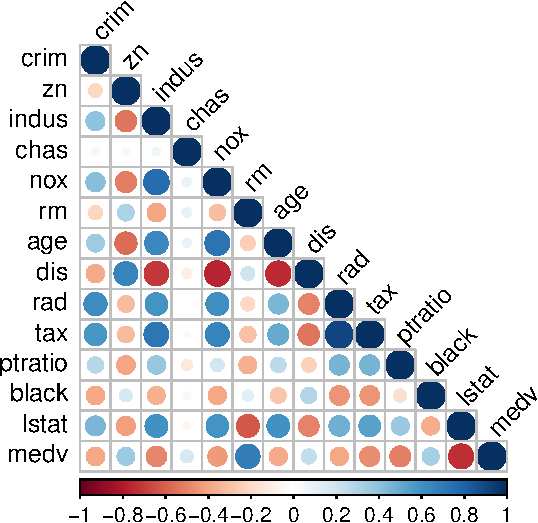
\includegraphics{HW3_files/figure-latex/unnamed-chunk-1-1} 

}

\caption{Correlation Matrix Intensity}\label{fig:unnamed-chunk-1}
\end{figure}

~

From the above correlation plot we can infer that crime is very loosely
related to `chas',`zn' and `rm'. We can also deduce that `chas' has
negligible magnitude while `zn' and `rm' has very less but more
magnitude than `chas'. So we will work on three subsets: (a)With all the
variables (b) Excluding `chas' (c) Excluding `chas', `zn' and `rm'

\newpage

\subsubsection{USING LOGISTIC
REGRESSION}\label{using-logistic-regression}

\subsubsection{Including all variables}\label{including-all-variables}

\begin{verbatim}
## Confusion Matrix for test data:
\end{verbatim}

\begin{verbatim}
##                 
## logi.test.pred_a  0  1
##                0 62  7
##                1  3 54
\end{verbatim}

\begin{verbatim}
## Train Accuracy:  0.9105263
\end{verbatim}

\begin{verbatim}
## Test Accuracy:  0.9206349
\end{verbatim}

~

\subsubsection{\texorpdfstring{Excluding
`chas'}{Excluding chas}}\label{excluding-chas}

\begin{verbatim}
## Confusion Matrix for test data:
\end{verbatim}

\begin{verbatim}
##                 
## logi.test.pred_b  0  1
##                0 61  7
##                1  4 54
\end{verbatim}

\begin{verbatim}
## Train Accuracy:  0.9105263
\end{verbatim}

\begin{verbatim}
## Test Accuracy:  0.9126984
\end{verbatim}

~

~

\subsubsection{\texorpdfstring{Excluding `chas', `rm',
`tax'}{Excluding chas, rm, tax}}\label{excluding-chas-rm-tax}

\begin{verbatim}
## Confusion Matrix:
\end{verbatim}

\begin{verbatim}
##                 
## logi.test.pred_c  0  1
##                0 61  8
##                1  4 53
\end{verbatim}

\begin{verbatim}
## Train Accuracy:  0.9131579
\end{verbatim}

\begin{verbatim}
## Test Accuracy:  0.9047619
\end{verbatim}

~

\newpage

\subsubsection{USING LDA}\label{using-lda}

\subsubsection{Including all variables}\label{including-all-variables-1}

\begin{verbatim}
## Confusion Matrix for test data:
\end{verbatim}

\begin{verbatim}
##    
##      0  1
##   0 62 15
##   1  3 46
\end{verbatim}

\begin{verbatim}
## Training Accuracy:  0.8571429
\end{verbatim}

\begin{verbatim}
## Test Accuracy:  0.8571429
\end{verbatim}

~

\subsubsection{\texorpdfstring{Excluding
`chas'}{Excluding chas}}\label{excluding-chas-1}

\begin{verbatim}
## Confusion Matrix for test data:
\end{verbatim}

\begin{verbatim}
##    
##      0  1
##   0 62 15
##   1  3 46
\end{verbatim}

\begin{verbatim}
## Training Accuracy:  0.8736842
\end{verbatim}

\begin{verbatim}
## Test Accuracy:  0.8571429
\end{verbatim}

~

\subsubsection{\texorpdfstring{Excluding `chas', `rm',
`tax'}{Excluding chas, rm, tax}}\label{excluding-chas-rm-tax-1}

\begin{verbatim}
## Confusion Matrix for test data :
\end{verbatim}

\begin{verbatim}
##    
##      0  1
##   0 64 15
##   1  1 46
\end{verbatim}

\begin{verbatim}
## Training Accuracy : 0.8631579
\end{verbatim}

\begin{verbatim}
## Test Accuracy, excluding chas, tax, rm:  0.8730159
\end{verbatim}

~

\newpage

\subsubsection{USING kNN}\label{using-knn}

\subsubsection{Including all variables}\label{including-all-variables-2}

\begin{verbatim}
## #kNN MODEL; including all variables
\end{verbatim}

\begin{verbatim}
## Confusion Matrix for test data :
\end{verbatim}

\begin{verbatim}
##           
## knn.pred_a  0  1
##          0 64  9
##          1  1 52
\end{verbatim}

\begin{verbatim}
## kNN Test Accuracy, including all variables:  0.9206349
\end{verbatim}

~

\subsubsection{\texorpdfstring{Excluding
`chas'}{Excluding chas}}\label{excluding-chas-2}

\begin{verbatim}
## #kNN MODEL; excluding 'chas'
\end{verbatim}

\begin{verbatim}
## Confusion Matrix for test data :
\end{verbatim}

\begin{verbatim}
##           
## knn.pred_b  0  1
##          0 64  9
##          1  1 52
\end{verbatim}

\begin{verbatim}
## Test Accuracy:  0.9206349
\end{verbatim}

~

\subsubsection{\texorpdfstring{Excluding `chas', `rm',
`tax'}{Excluding chas, rm, tax}}\label{excluding-chas-rm-tax-2}

\begin{verbatim}
## #kNN MODEL; excluding 'chas', 'rm', 'tax'
\end{verbatim}

\begin{verbatim}
## Confusion Matrix for test data :
\end{verbatim}

\begin{verbatim}
##           
## knn.pred_c  0  1
##          0 57 12
##          1  8 49
\end{verbatim}

\begin{verbatim}
## Test Accuracy:  0.8412698
\end{verbatim}

\subsubsection{INFERENCES :}\label{inferences}

From the above computations, we see that the performance of logistic
regression and knn is better than the LDA classification method. This
maybe because the predictors are not normally distributed and also
because the classes not linearly seperable. Although there is some
difference in the performance of the LDA, it is not very pronounced.
\newpage

\subsection{SOLUTION 2}\label{solution-2}

\subsubsection{(a)}\label{a}

When we look at the pairplot below we can see that most of the
distributions are different for each of the plot. Hence each class will
have different covariance with respect to the pairwise variables and
eventually will have different covariance matrices. \newline

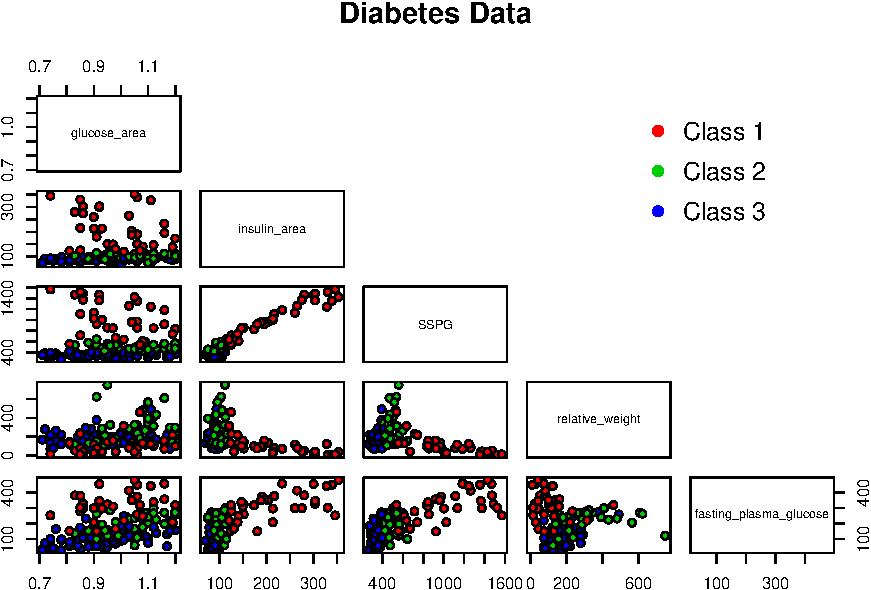
\includegraphics{HW3_files/figure-latex/unnamed-chunk-11-1.pdf}

Its hard to determine if each class have a multivariate distribution.
So, we'll do a multivariate test using MVN library to check if the
classes have multivariate distribution.

\begin{verbatim}
## sROC 0.1-2 loaded
\end{verbatim}

\begin{verbatim}
## Multivariate test for class 1
\end{verbatim}

\begin{verbatim}
##              Test         Statistic              p value Result
## 1 Mardia Skewness  72.1130242128528 0.000223018134108012     NO
## 2 Mardia Kurtosis 0.759602021039537    0.447492510707829    YES
## 3             MVN              <NA>                 <NA>     NO
\end{verbatim}

\begin{verbatim}
## Multivariate test for class 2
\end{verbatim}

\begin{verbatim}
##              Test          Statistic            p value Result
## 1 Mardia Skewness   50.8434201071473 0.0406859141683021     NO
## 2 Mardia Kurtosis 0.0757723206589703  0.939600237713607    YES
## 3             MVN               <NA>               <NA>     NO
\end{verbatim}

\begin{verbatim}
## Multivariate test for class 3
\end{verbatim}

\begin{verbatim}
##              Test        Statistic             p value Result
## 1 Mardia Skewness 68.2997291313893 0.00063808969256816     NO
## 2 Mardia Kurtosis 2.08698632017701  0.0368893711399998     NO
## 3             MVN             <NA>                <NA>     NO
\end{verbatim}

From the above test we can see that class 1 and 2 passes just Mardia
Kurtosis test but fails the Mardia Skewness test. While class 3 fails
both the test. So we conclude that the classes does not have
multivariate distribution. But as we have very less data points, our
conclusion are not with confidence.

~

\subsubsection{(b)}\label{b}

\begin{verbatim}
## FITTING LDA MODEL:
\end{verbatim}

\begin{verbatim}
## Confusion Matrix for test data:
\end{verbatim}

\begin{verbatim}
##    
##      1  2  3
##   1  8  0  0
##   2  2 10  0
##   3  1  0 15
\end{verbatim}

\begin{verbatim}
## Training Accuracy : 0.9082569
\end{verbatim}

\begin{verbatim}
## Test Accuracy :  0.9166667
\end{verbatim}

\begin{verbatim}
## FITTING QDA MODEL:
\end{verbatim}

\begin{verbatim}
## QDA Confusion Matrix for test data:
\end{verbatim}

\begin{verbatim}
##    
##      1  2  3
##   1  9  0  0
##   2  2  9  0
##   3  0  1 15
\end{verbatim}

\begin{verbatim}
## QDA Training Accuracy : 0.9541284
\end{verbatim}

\begin{verbatim}
## QDA Test Accuracy :  0.9166667
\end{verbatim}

\subsubsection{(c)}\label{c}

\begin{verbatim}
## The posterior probabilities for the data is :
\end{verbatim}

\begin{verbatim}
##              1         2         3
## 1 4.841209e-05 0.5462818 0.4536698
\end{verbatim}

\begin{verbatim}
## And the class predicted by QDA is :  2
\end{verbatim}

\begin{verbatim}
## The posterior probabilities for the data is :
\end{verbatim}

\begin{verbatim}
##           1         2            3
## 1 0.2214092 0.7785877 3.117562e-06
\end{verbatim}

\begin{verbatim}
## And the class predicted by QDA is :  2
\end{verbatim}

~


\end{document}
